\chapter{The iPhone application}
\lettrine[lines=4, loversize=-0.1, lraise=0.1]{L}{orem ipsum dolor} sit amet, consectetur adipiscing elit. Donec viverra gravida adipiscing.


\section{PhraseDroid}
\subsection{Sub-header}


\section{iPhrase}
The developed iPhone application can roughly be divided into two parts. There is the user interface to provide interactivity and present results, and the Grammarian that interfaces with libpgf+.


\subsection{Grammarian}
\label{sec:grammarian}
The Grammarian class is the glue between the C++ api of libpgf+ and the Objective C code in the rest of the application. It provides methods to enumerate available languages, to translate between three-letter languages codes and full language names, and most importantly to parse input, generate translations and predict continuations of the current input. The public interface of the class is shown in listing \ref{lst:grammarian}.

The enumeration of available languages is done by querying libpgf+ for the list of concrete syntaxes for the current grammar. These names are not very user friendly though. Therefor a method to generate a human readable name is provided. This method extracts the three letter code at the end of the concrete syntax name and looks it up in a table with all the ISO 639 language codes and their corresponding language names.

Parsing is done by accepting one token at a time and passing it on to libpgf+, keeping a reference to the current parser state in the grammarian. This state is then queried for predictions which are cached until needed.

Translations are generated by asking the current parser state for all available parse trees and then handing them over to the concrete syntax of the grammar corresponding to the requested target language. The resulting linearisations are then returned to the caller.

There are two methods to predict continuations. The first method uses simple prefix matching on the list of cached predictions. The second method calculates the Damerau–Levenshtein distance between the supplied string and each token, and only returns those tokens that either has the supplied string as a prefix or has an edit distance less than or equal to the supplied number.

\lstinputlisting[language={[Objective]C}, frame=single, breaklines=true, float, captionpos=b, linerange={11-35}, caption=Public interface of the Grammarian class., label=lst:grammarian]{../iPhrase/iPhrase/Grammarian.h}



\subsection{User interface}
The user interface of the application consists of five different views that can be accessed through the flow shown in \ref{fig:storyboard}. The starting view is the input view. The main part of this view is occupied by the token input and the keyboard. At the top of the view are two buttons to transition to either the settings view or the translations view. The translation button is only available if the current input can be parsed to a top level production by the grammar.

\begin{figure}[htb]
\centering
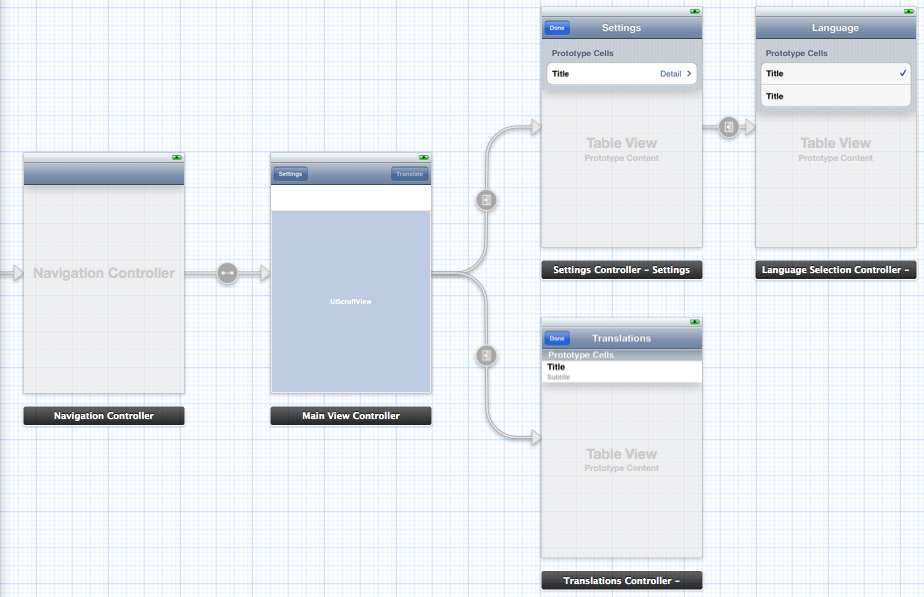
\includegraphics[width=0.8\textwidth]{fig/storyboard}
\caption{UI flow}
\label{fig:storyboard}
\end{figure}


\subsubsection{Token input}
Token input can be done in two ways. One way is to touch one of the token buttons shown in the token input view. The other way is to enter text manually into the provided text field.

The token input view shows the possible continuations of the current input. The list of possible tokens is provided by the Grammarian as described in \ref{sec:grammarian}. A button is created for each token. The buttons are then laid out to fit in the current width of the token main input view as seen in figures \ref{fig:inputview_portrait} and \ref{fig:inputview_landscape}. The height of the token input view is then adjusted to fit all the buttons to enable scrolling in the parent view.

\begin{figure}[htb]
\centering
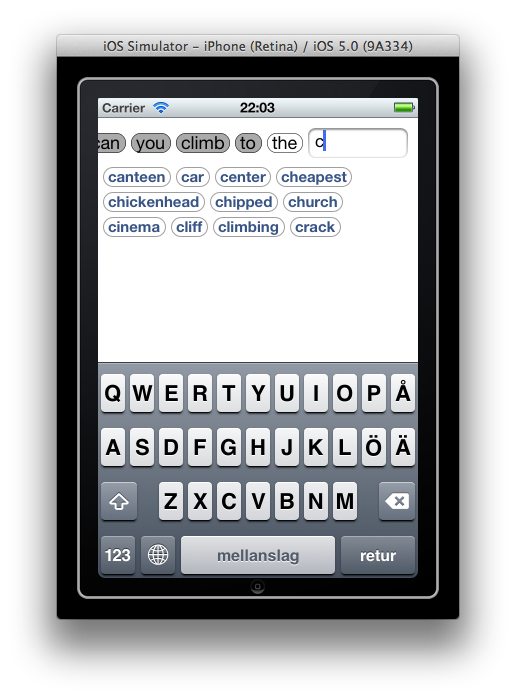
\includegraphics[width=0.8\textwidth]{fig/inputview_portrait}
\caption{Input view (portrait)}
\label{fig:inputview_portrait}
\end{figure}

\begin{figure}[htb]
\centering
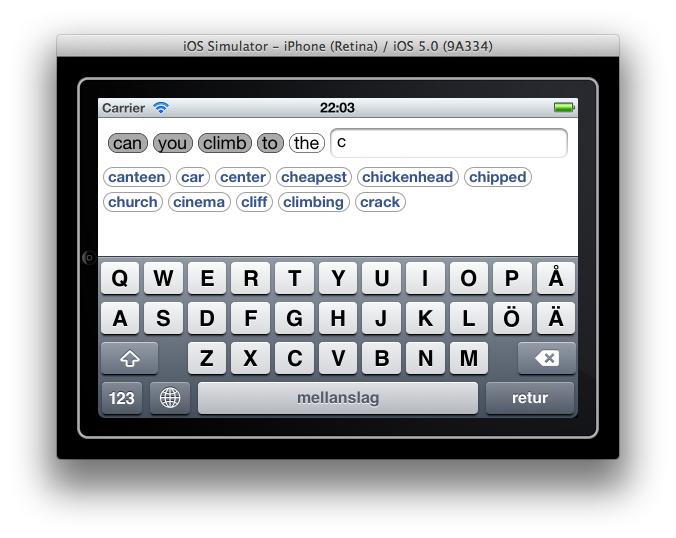
\includegraphics[width=0.8\textwidth]{fig/inputview_landscape}
\caption{Input view (landscape)}
\label{fig:inputview_landscape}
\end{figure}

Touching a token will tell the advance the grammarian using the corresponding token, after which the token input view will be updated to reflect the newly available predictions.

When the grammarian is advanced the new token will also be added to a list of processed tokens along with a corresponding button visible at the top of the token input just left of the input text field.

If text is entered into the text field the entered text will be used as a prefix to limit the list of tokens returned by the grammarian. If no tokens are returned, a second query for tokens is performed but this time with an allowed maximum edit distance of one as explained in \ref{sec:grammarian}. This is to make allowances for the user misspelling a token.

If a space is entered and the current text is a valid token or has a maximum edit distance of one from one and only one valid token the grammarian is advaned as if the corresponding token button had been touched.

If the text field is empty and a back space is entered, the previous input token will be removed from the list of processed tokens and instead be placed in the text field. This same effect can also be achieved by touching the button corresponding to the last processed token.


\subsubsection{Translations}
The translations view shows a list of the generated translations for the given input and also a using a disambiguation concrete syntax if the current grammar supports it. Touching any of the translations will take the user to the translation details view. The translations view, like the settings view, features a button to return to the input view.


\subsubsection{Translation details}
The translation details view shows the full text of the translation and below it the full text of the disambiguation if available. There is also a back button to return to the translations view.


\subsubsection{Settings}
The settings view shows a list of the available options in the application. Currently this is the from and to languages for the translation. Touching one of these will take the user to the language selection view. The settings view also features a button to return to the input view.


\subsubsection{Language selection}
The language selection view dynamically creates a list of all the languages available in the current grammar. The active language has a mark to indicate it is in use. Touching any of the languages in the list will make that language active for the current setting (to/from) and return to the settings view. There is also a back button to return to the settings view without changing the active language.


\subsection{Reusability}
The grammar used in the application is loaded from a PGF file. This allows the grammar to be replaced without having to change the whole application.
